\documentclass[journal]{IEEEtran}
\usepackage[a5paper, margin=10mm]{geometry}
%\usepackage{lmodern} % Ensure lmodern is loaded for pdflatex
\usepackage{tfrupee} % Include tfrupee package


\setlength{\headheight}{1cm} % Set the height of the header box
\setlength{\headsep}{0mm}     % Set the distance between the header box and the top of the text


%\usepackage[a5paper, top=10mm, bottom=10mm, left=10mm, right=10mm]{geometry}

%
\setlength{\intextsep}{10pt} % Space between text and floats

\makeindex


\usepackage{cite}
\usepackage{amsmath,amssymb,amsfonts,amsthm}
\usepackage{algorithmic}
\usepackage{graphicx}
\usepackage{textcomp}
\usepackage{xcolor}
\usepackage{txfonts}
\usepackage{listings}
\usepackage{enumitem}
\usepackage{mathtools}
\usepackage{gensymb}
\usepackage{comment}
\usepackage[breaklinks=true]{hyperref}
\usepackage{tkz-euclide} 
\usepackage{listings}
\usepackage{multicol}
\usepackage{xparse}
\usepackage{gvv}
%\def\inputGnumericTable{}                                 
\usepackage[latin1]{inputenc}                                
\usepackage{color}                                            
\usepackage{array}                                            
\usepackage{longtable}                                       
\usepackage{calc}                                             
\usepackage{multirow}                                         
\usepackage{hhline}                                           
\usepackage{ifthen}                                               
\usepackage{lscape}
\usepackage{tabularx}
\usepackage{array}
\usepackage{float}
\usepackage{ar}
\usepackage[version=4]{mhchem}


\newtheorem{theorem}{Theorem}[section]
\newtheorem{problem}{Problem}
\newtheorem{proposition}{Proposition}[section]
\newtheorem{lemma}{Lemma}[section]
\newtheorem{corollary}[theorem]{Corollary}
\newtheorem{example}{Example}[section]
\newtheorem{definition}[problem]{Definition}
\newcommand{\BEQA}{\begin{eqnarray}}
\newcommand{\EEQA}{\end{eqnarray}}

\theoremstyle{remark}


\begin{document}
\bibliographystyle{IEEEtran}
\onecolumn

\title{METALLURGY ENGINEERING}
\author{GATE 2013\\
EE25BTECH11027-INDHIRESH S}
\maketitle


\renewcommand{\thefigure}{\theenumi}
\renewcommand{\thetable}{\theenumi}

\section{Q1 - Q25 carry one mark each}
\begin{enumerate}
\item  Degree and order of the differential equation $\frac{d^2y}{dx^2} + 3\frac{dy}{dx}-6y =0$, respectively, are \hfill{\brak{\text{GATE MT 2013}}}

\begin{multicols}{4}
\begin{enumerate}
\item $1\; \text{and}\; 2$ 
\item  $2 \;\text{and}\; 1$ 
\item $1 \;\text{and}\; 1$ 
\item $2 \;\text{and}\; 2$ 
\end{enumerate}
\end{multicols}

\item  As the concentration of point defects in a crystal increases, its configurational entropy
\hfill{\brak{\text{GATE MT 2013}}}
\begin{multicols}{2}
\begin{enumerate}
\item does not change 
\item  decreases 
\item increases 
\item initially increases and then decreases 
\end{enumerate}
\end{multicols}

\item In a binary system $A-B$, $\epsilon_{AA}$, $\epsilon_{BB}$ and $\epsilon_{AB}$ correspond to $A-A, B-B\; \text{and}\; A-B$ bond energies respectively. The miscibility gap will occur if 
\hfill{\brak{\text{GATE MT 2013}}}
\begin{multicols}{2}
\begin{enumerate}
\item $\epsilon_{AB} > \frac{1}{2} (\epsilon_{AA} + \epsilon_{BB}) $
\item  $\epsilon_{AB} < \frac{1}{2} (\epsilon_{AA} + \epsilon_{BB}) $
\item $\epsilon_{AB} = \frac{1}{2} (\epsilon_{AA} + \epsilon_{BB}) $
\item  $\epsilon_{AB} < \frac{1}{4} (\epsilon_{AA} + \epsilon_{BB}) $
\end{enumerate}
\end{multicols}

\item  Critical value of the Gibbs energy of nucleation at equilibrium temperature is \hfill{\brak{\text{GATE MT 2013}}}

\begin {multicols}{4}
\begin{enumerate}
\item zero 
\item  infinite 
\item  positive
\item negative 
\end{enumerate}
\end{multicols}

\item  With respect to the matrix of Al-Cu alloys, $G-P$ zones are 
\hfill{\brak{\text{GATE MT 2013}}}
\begin{multicols}{2}
\begin{enumerate}
\item coherent 
\item incoherent
\item  semi-coherent
\item chemically indistinguishable 
\end{enumerate}
\end{multicols}

\item  Which one of the following techniques does NOT require quenching to obtain final case hardness? \hfill{\brak{\text{GATE MT 2013}}}
\begin{multicols}{2}
    

\begin{enumerate}
\item Flame hardening 
\item Induction hardening
\item  Nitriding
\item Carburizing
\end{enumerate}
\end{multicols}

\item Which one of the following elements is an austenite stabilizer? 
 \hfill{\brak{\text{GATE MT 2013}}}
\begin{multicols}{4}
\begin{enumerate}
\item Nitrogen 
\item  Molybdenum
\item  Vanadium 
\item Tungsten 
\end{enumerate}
\end{multicols}

\item A $0.2 wt\%$ plain carbon steel sheet is heated and equilibrated in the inter-critical region followed by instant water quenching. The microstructure of the quenched steel sheet consists of\hfill{\brak{\text{GATE MT 2013}}}
\begin{multicols}{2}
\begin{enumerate}
\item fully martensite 
\item $\text{proeutectoid ferrite} + \text{pearlite} $
\item $\text{martensite} + \text{pearlite } $  
\item $\text{martensite} + \text{austenite } $

\end{enumerate}
\end{multicols}

\item As compared to the engineering stress-engineering strain curve, the true stress-true strain curve for a given material  \hfill{\brak{\text{GATE MT 2013}}}
\begin{enumerate}
\item lies above and to the left
\item  lies below and to the right
\item  crosses the engineering stress-engineering strain curve 
\item  is identical 
\end{enumerate}

\item Which one of the following does NOT improve fatigue life of a steel component? 

\hfill{\brak{\text{GATE MT 2013}}}
\begin{multicols}{2}
\begin{enumerate}
\item Nitriding 
\item Decarburization 
\item  Improving surface finish
\item Shot-peening    
\end{enumerate}
\end{multicols}
\item When two phases $\alpha$ and $\beta$ in an alloy are in thermodynamic equilibrium, then\hfill{\brak{\text{GATE MT 2013}}}
\begin{multicols}{4}
\begin{enumerate}
        \item $C_p^\alpha=C_p^\beta$
        \item $V_m^\alpha=V_M^\beta$
        \item $G_m^\alpha=G_m^\beta$
        \item $\overline{G_i^\alpha} = \overline{G_i^\beta}$
\end{enumerate}
\end{multicols}
\item Isothermal compressibility of a material is given by \hfill{\brak{\text{GATE MT 2013}}}

\begin{multicols}{4}
\begin{enumerate}
    \item $-\frac{1}{p}(\frac{\partial V}{\partial p})_T$
    \item $\frac{1}{p}(\frac{\partial V}{\partial p})_T$
    \item$-\frac{1}{V}(\frac{\partial V}{\partial p})_T$
    \item $\frac{1}{V}(\frac{\partial V}{\partial p})_T$
\end{enumerate}
\end{multicols}
\item In the Ellingham diagram for oxides, $C-CO$ line cuts the $M-MO$ line at temperature $T_1$ and the $M'-M$ line at a higher temperature $T_2$. At a temperature greater than $T_1$ and less than $T_2$, carbon
can reduce\\
\hfill{\brak{\text{GATE MT 2013}}}
\begin{multicols}{2}
\begin{enumerate}
    \item $MO$
    \item both $MO\; \text{and} \; M'O$
    \item $M'O$
    \item neither $MO\; \text{nor} \;M'O$ 
\end{enumerate}
    
\end{multicols}


\item Which one of the following can give information about the corrosion rate?\hfill{\brak{\text{GATE MT 2013}}}

\begin{multicols}{2}
\begin{enumerate}
\item Pourbaix diagram 
\item Polarization technique 
\item EMF series 
\item  Galvanic series 
\end{enumerate}
\end{multicols}

\item In a roasting process, the set of conditions that favour sulphate formation from metal sulphide concentrates are 
\begin{enumerate}[label=\Alph*), start=16]

\item high temperature
\item high partial pressure of oxygen
\item use of excess air 
\item use of excess air 
\end{enumerate}
\hfill{\brak{\text{GATE MT 2013}}}
\begin{multicols}{4}
\begin{enumerate}
\item $P, R\; and \;S$
\item $P, Q\; and\; R$
\item  $Q\; and\; S$ 
\item $R\; and \;S $
\end{enumerate}
\end{multicols}

\item  High top pressure in a blast furnace operation

\begin {multicols}{2}
\begin{enumerate}
\item  favours the solution-loss reaction
\item suppresses the solution-loss reaction 
\item  decreases gas-solid contact time 
\item increases coke rate 

\end{enumerate}
\end{multicols}

\item In L-D steelmaking, the final slag can be best described as 
\hfill{\brak{\text{GATE MT 2013}}}
\begin{enumerate}
\begin{multicols}{2}
    

\item oxidizing 
\item basic
\item oxidizing and basic 
\item reducing and basic
\end{multicols}
\end{enumerate}

\item  The permeability of burden in an ironmaking blast furnace can be improved by using \hfill{\brak{\text{GATE MT 2013}}}
\begin{enumerate}
\item fine charge
\item agglomerated charge
\item oxygen enriched air blast
\item pulverized coal injection through the tuyeres
\end{enumerate}

\item For a good quality brazing, the molten filler alloy should have \hfill{\brak{\text{GATE MT 2013}}}
\begin{multicols}{2}
\begin{enumerate}
\item low contact angle with the base metal
\item low density 
\item high surface tension 
\item high viscosity 
\end{enumerate}
\end{multicols}

\item Risers are NOT required for casting 
\hfill{\brak{\text{GATE MT 2013}}}
\begin{multicols}{2}
\begin{enumerate}
\item stainless steel 
\item plain carbon steel 
\item grey cast iron
\item white cast iron 
\end{enumerate}
\end{multicols}

\item For scalar fields $\phi$ and $\psi$, the value of $\nabla.(\nabla\phi\times\nabla\psi)$ is\underline {\hspace{2cm}}\hfill{\brak{\text{GATE MT 2013}}}

\item The atomic packing fraction of diamond cubic structure is\underline {\hspace{2cm}}\\
\hfill{\brak{\text{GATE MT 2013}}}\\

\item The total number of possible heat transfer mode(s) is \underline {\hspace{2cm}}                \hfill{\brak{\text{GATE MT 2013}}}\\

\item If $\sigma$ and $\epsilon$ are true stress and true strain, respectively, the maximum true uniform strain that can be
imparted to a material obeying $\sigma=1050\epsilon^{0.25}$ is \underline {\hspace{2cm}} \hfill{\brak{\text{GATE MT 2013}}}

\item  Arc welding is done using current, voltage and welding speed of $200 A, 20 V \;\text{and}\; 0.01 m/s$, respectively. The heat input in $kJ$ per unit length is \underline {\hspace{2cm}} \hfill{\brak{\text{GATE MT 2013}}}

\section{Q26 - Q55 carry two marks each}

\item  Which one of the following series is divergent?\hfill{\brak{\text{GATE MT 2013}}}
\begin{multicols}{4}
\begin{enumerate}
\item $\sum_{n=1}^\infty \frac{1}{3^{n-1}}$
\item $\sum_{n=1}^\infty \frac{1}{n}$
\item $\sum_{n=0}^\infty \frac{1}{2^{n}}$
\item $\sum_{n=1}^\infty \frac{1}{n^{n}}$
\end{enumerate}
\end{multicols}

\item Taylor series expansion of the function $f(x)=\frac{x}{1+x}$ around $x=0$ will be
\hfill{\brak{\text{GATE MT 2013}}}
\begin{multicols}{4}
\begin{enumerate}
\item $1+x+x^2+x^3+...$
\item $1-x+x^2-x^3+...$
\item $0+x+\frac{x^2}{2}+\frac{x^3}{3}+...$
\item $0+x-x^2+x^3-...$
\end{enumerate}
\end{multicols}

\item  Which one of the following attributes is NOT correct for the matrix? 
 \hfill{\brak{\text{GATE MT 2013}}}\\
 \begin{align}
\myvec{\cos{\theta}& -\cos{\theta} & 0\\ \sin{\theta}& \cos{\theta}& 0\\ 0& 0 & 1
 } , \text{where}\; \theta=60\degree
  \end{align}

\begin {multicols}{4}
\begin{enumerate}
\item orthogonal
\item  singular 
\item skew-symmetric 
\item positive-definite 
\end{enumerate}
\end{multicols}

\item A unit cell of an element has maximum linear density along the $[110]$ direction. The packing density of its $(100)$ plane is
\hfill{\brak{\text{GATE MT 2013}}}
\begin{multicols}{4}
\begin{enumerate}
\item  $0.68$
\item  $0.74 $
\item $0.79$ 
\item $0.91$
\end{enumerate}
\end{multicols}

\item For an FCC metal, the ratio of interplanar spacing obtained from the first two peaks of the X-ray diffraction pattern is  \hfill{\brak{\text{GATE MT 2013}}}
\begin{multicols}{4}
\begin{enumerate}
\item  $1.91$
\item  $1.63$ 
\item $1.41$ 
\item $1.15 $
\end{enumerate}
\end{multicols}

\item There are $150$ gearwheels in a box, out of which $112$ are within the required tolerance, $21$ are below and rest are above the required tolerance. If the selection is done without replacement, the combined probability of randomly selecting a gearwheel below the tolerance and then a second one above the tolerance is   \hfill{\brak{\text{GATE MT 2013}}}
\begin{multicols}{4}
\begin{enumerate}
\item $0.016 $
\item  $0.032$ 
\item $0.492$
\item $0.984$ 
\end{enumerate}
\end{multicols}
\item Match the metal in Group 1 with its corresponding ore in Group 2\hfill{\brak{\text{GATE MT 2013}}}
\begin{center}
\begin{tabular}{ll}
\textbf{Group 1 }    &  \textbf{Group 2}\\
P.  Ni      &1. Monazite\\
Q. Th  &2. Cassiterite\\ 
R. Pb  &3. Penlandite \\
S.Sn  & 4.Galena 
\end{tabular}
\end{center}
\begin{multicols}{2}
\begin{enumerate}
\item  $P-1, Q-3, R-4, S-2$
\item $P-4, Q-2, R-3, S-1$ 
\item  $P-3, Q-1, R-4, S-2$ 
\item $P-2, Q-3, R-1, S-4$
\end{enumerate}
\end{multicols}

\item The yield strength of a polycrystalline metal increases from $100 MPa$ to $145 MPa$ on decreasing the grain size from $64 \micro m$ to $25 \micro m$. The yield strength of this metal (in MPa) having a grain size of $36\micro m$ is
\hfill{\brak{\text{GATE MT 2013}}}
\begin{multicols}{4}
\begin{enumerate}
\item $110$ 
\item  $125$
\item $140$
\item $165$ 
\end{enumerate}
\end{multicols}

\item  In a brittle material, the maximum internal crack length is $8 \micro m$. If Young's modulus is $400 GPa$ and surface energy is $3.14 J/m^2$ , the estimated theoretical fracture strength (in MPa) is \hfill{\brak{\text{GATE MT 2013}}}
\begin{multicols}{4}
    \begin{enumerate}
    \item  $375$
    \item  $412$
    \item  $327$
    \item  $447$  
\end{enumerate}
\end{multicols}
\item Saturation magnetization of an FCC metal with lattice parameter $0.2 nm$ is $600 kA/m$. The net magnetic moment per atom is given by (in Bohr magneton)\hfill{\brak{\text{GATE MT 2013}}}

\begin{multicols}{4}
\begin{enumerate}
        \item $8.08 \times 10^{57}$
        \item  $2.02\times 10^{57}$
        \item  $0.517$ 
        \item $0.129$
\end{enumerate}
\end{multicols}
\item  A $480 mm$ thick slab is hot-rolled using a roll of $720 mm$ diameter. For a coefficient of friction of $0.5$, the maximum possible reduction (in mm) is \hfill{\brak{\text{GATE MT 2013}}}

\begin{multicols}{4}
\begin{enumerate}
    \item  $90$ 
    \item $180 $
    \item $240$ 
    \item $360 $

\end{enumerate}
\end{multicols}
\item Match the defects listed in Group I with the corresponding manufacturing process listed in Group II.
\hfill{\brak{\text{GATE MT 2013}}}\\
\begin{center}
\begin{tabular}{ll}
\textbf{Group 1} & \textbf{Group 2}\\
  (P) Orange-peel effect    & (1) Extrusion \\
   (Q) Chevron cracking   & (2) Deep drawing \\
   (R) Flash & (3) Arc welding \\
   (S) Undercut & (4) Forging \\
\end{tabular}
\end{center}
\begin{multicols}{2}
    

\begin{enumerate}
    \item $P-1, Q-2, R-4, S-3 $
    \item  $P-2, Q-3, R-1, S-4$
    \item $P-3, Q-4, R-2, S-4$
    \item $P-2, Q-1, R-4, S-3 $
\end{enumerate}
\end{multicols}



\item Match the powder production technique given in Group I with the corresponding shape listed in \hfill{\brak{\text{GATE MT 2013}}}\\
\begin{center}
\begin{tabular}{ll}
\textbf{Group 1 }& \textbf{Group 2}\\
 (P) Reduction     &  (1) Flaky \\
  (Q) Gas Atomization    & (2) Spongy \\
 (R) Milling & (3) Dendritic\\
 (S) Electrolysis & (4) Spherical\\
\end{tabular}
\end{center}
\begin{multicols}{2}
\begin{enumerate}
\item $P-2, Q-4, R-1, S-3$
\item  $P-1, Q-3, R-2, S-4$ 
\item $P-2, Q-3, R-4, S-1$
\item  $P-3, Q-2, R-1, S-4$
\end{enumerate}
\end{multicols}

\item Match the suitability of non-destructive testing method in Group I for the detection of defects listed in Group II \hfill{\brak{\text{GATE MT 2013}}}\\
\begin{center}
    

\begin{tabular}{ll}
\textbf{Group 1} & \textbf{Group 2} \\
 (P) Magnetic particle inspection      &  (1) Surface crack in martensitic stainless steels  \\
  (Q) X-ray radiography    & (2) Surface crack in austenitic stainless steels \\
 (R) Dye penetrant test & (3) Hairline crack in aluminium \\
 (S) Ultrasonic testing  & (4) Inclusions in steels \\
\end{tabular}
\end{center}
\begin{multicols}{2}
\begin{enumerate}
\item  $P-2, Q-4, R-3, S-1$
\item  $P-4, Q-2, R-1, S-3$ 
\item  $P-3, Q-1, R-2, S-4$
\item   $P-1, Q-4, R-2, S-3$ 
\end{enumerate}
\end{multicols}

\item For the following electrochemical reaction $Sn + 2H^+
 = Sn^{2+} + H_2$, if the solution has $Sn^{2+}$ concentration $10^{-2}$ M and $pH \;5$ at $298 K$, which of the following is true?
Given: standard reduction potential for $Sn^{2+} + 2e^- \longrightarrow Sn$ is $-0.136 V\; \text{versus}$ SHE; $p_{H_2} = 1 atm$\hfill{\brak{\text{GATE MT 2013}}}


\begin{multicols}{2}

\begin{enumerate}
\item   Sn undergoes oxidation
\item  $H^+$ undergoes reduction
\item   $Sn^{2+}$ undergoes reduction
\item  No net reaction
\end{enumerate}
\end{multicols}
\item Match the unit operation in Group I with its corresponding principle in Group II: \hfill{\brak{\text{GATE MT 2013}}}\\
\begin{center}
    

\begin{tabular}{ll}
\textbf{Group 1 }& \textbf{Group 2} \\
 (P) Jigging      &  (1) Modification of surface tension \\
  (Q) Tabling    & (2) Difference in density\\
 (R) Heavy media separation & (3) Differential initial acceleration  \\
 (S) Flotation & (4) Differential lateral movement \\
\end{tabular}
\end{center}
\begin{multicols}{2}
\begin{enumerate}
\item   $P-3, Q-4, R-2, S-1$
\item  $P-2, Q-3, R-1, S-4$ 
\item   $P-4, Q-2, R-3, S-1$ 
\item   $P-1, Q-3, R-2, S-4$
\end{enumerate}
\end{multicols}

\item  Determine the correctness or otherwise of the following Assertion (a) and Reason (r). \hfill{\brak{\text{GATE MT 2013}}}\\
Assertion: For the extraction of metal values from their sulphide concentrates by
hydrometallurgical route, leaching with oxygen under high pressure is used. \\
Reason:Presence of oxygen under high pressure causes roasting of sulphides, which helps in leaching of the values. \\


\begin{enumerate}
\item  a is true but r is false
\item  a is false but r is true
\item  both a and r are true, and r is the reason for a
\item  both a and r are true, but r is not the reason for a
\end{enumerate}

\item The aperture size $(in \micro m)$ of a $200$ mesh sieve having a wire diameter of $53 \micro m$ is \underline {\hspace{2cm}} \hfill{\brak{\text{GATE MT 2013}}}\\


\item From a $2 m \times 1.2 m $sheet, squares are cut out from each of the four corners as shown in the figure and then the sides are bent to form an open box. The maximum possible volume $(\text{in}\; m^3 )$ of the box is \underline {\hspace{2cm}} \hfill{\brak{\text{GATE MT 2013}}}\\

\begin{figure}[H]
    \centering
    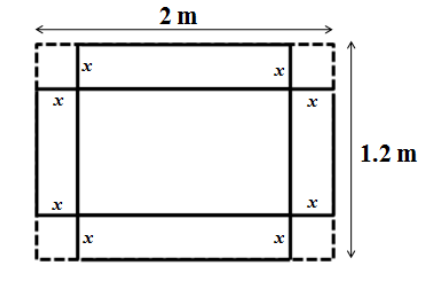
\includegraphics[width=0.5\columnwidth]{figs/Q.44.png}
    \caption\centering{CUTTED SHEET}
    \label{fig:placeholder}
\end{figure}


	\item  Applying the secant method, the first approximation to the root of $f(x)=1+\ln{x}+\frac{x}{2}$ starting
with function values at $x = 0.3\; \text{and}\; x=0.4$, is \underline {\hspace{2cm}}
    \hfill{\brak{\text{GATE MT 2013}}}\\


\item  The critical internal crack length (in mm) in a steel having $K_{I_C}$ of $45MPa\sqrt{m}$ to support a Mode-I stress of $400 MPa$ is \underline {\hspace{2cm}}
 \hfill{\brak{\text{GATE MT 2013}}}


\item  Ladle deoxidation of liquid steel is done at $1600\degree C$ by adding ferro-aluminium. By assuming Stokes law behaviour, time (in s) required for alumina particles of $50\micro m$diameter to float to the surface from a depth of $2 m$ would be \underline {\hspace{2cm}}
\hfill{\brak{\text{GATE MT 2013}}}
\section*{Common Data Questions }
\subsection*{Common Data for Questions 48 and 49: }
A steel specimen containing $0.2 wt.\%$C is carburized in an atmosphere that maintains a carbon content of $1.2 wt.\%$ C at the surface of the specimen.
\begin{center}
\begin{tabular}{|c|c|}
\hline
\textbf{y} & \textbf{erf(y)} \\

\hline
0.85 & 0.7707 \\
0.90 & 0.7970 \\
0.95 & 0.8209 \\

\hline
\end{tabular}
\end{center}
\item   What is the depth $(in\; \micro m)$ from the surface of the specimen at which a composition of $0.4 wt.\%$ C is obtained after carburizing at $870\degree C$ for $10\; h$? 
\hfill{\brak{\text{GATE MT 2013}}}

\begin {multicols}{4}
\begin{enumerate}
\item$ 15 $
\item $ 84  kg$
\item  $113  kg$ 
\item  $ 875  kg$
\end{enumerate}
\end{multicols}

\item  How long (in h) will it take to double the depth at which $0.4 wt.\% C$ is reached? 
\hfill{\brak{\text{GATE MT 2013}}}
\begin{multicols}{4}
\begin{enumerate}
\item  $40 $
\item $20 $
\item $18 $
\item $ 14 $
\end{enumerate}
\end{multicols}
\subsection*{Common Data for Questions 50 and 51: }
Integral enthalpy of mixing (in J/mol) of liquid (Cu, Zn) solution can be approximated by $\Delta H^{mix}_m=-19250_{{x_{cu}}{x_{zn}}}$

\item The corresponding partial molar enthalpy of mixing (in J/mol) for Cu is \hfill{\brak{\text{GATE MT 2013}}}
\begin{multicols}{2}
\begin{enumerate}
\item $19250_{x^2_{Zn}}$
\item  $-19250_{x^2_{Cu}}$
\item  $38500_{x_{Zn}}- 19250_{x^2_{Zn}}-19250$
\item  $-19250_{x^2_{Zn}}$
\end{enumerate}
\end{multicols}
\item Assuming regular solution behaviour, the solution parameter (in J/mol) is \hfill{\brak{\text{GATE MT 2013}}}
\begin{multicols}{4}
\begin{enumerate}
\item $-19250 $
\item  $ -9625$
\item  $ 13.75 $
\item  $2315.4 $
\end{enumerate}
\end{multicols}
\section*{Linked Answer Questions }
\subsection*{Statement for Linked Answer Questions 52 and 53: }
The density and associated crystallinity for two polypropylene samples are as follows: 
\begin{center}
    \begin{tabular}{ll}
      \textbf{density, $g/cm^3$  } & \textbf{crystallinity, $\%$} \\
    $1.20$  & $50$ \\
     $1.44$ &  $80$ \\
    \end{tabular}
\end{center}
\item   Density of totally amorphous polypropylene is
\hfill{\brak{\text{GATE MT 2013}}}
\begin{multicols}{4}
\begin{enumerate}
\item    $0.64$
\item $0.74$
\item  $ 0.84$ 
\item $0.94$
\end{enumerate}
\end{multicols}

\item   The percent crystallinity of polypropylene sample having a density of $1.3 g/cm^3$  is
\hfill{\brak{\text{GATE MT 2013}}}

\begin {multicols}{4}
\begin{enumerate}
\item  $54$ 
\item  $64 $
\item $74$
\item  $84 $
\end{enumerate}
\end{multicols}
\subsection*{Statement for Linked Answer Questions 54 and 55: }
An edge dislocation is present in $\alpha-Fe$. Atomic diameter of iron atom is $0.25 nm$ and its shear modulus is $70 GPa$.

\item   Modulus of the Burgers vector (in nm) is
\hfill{\brak{\text{GATE MT 2013}}}
\begin {multicols}{4}
\begin{enumerate}
\item   $ 0.125 $
\item  $0.25$
\item   $ 0.50 $
\item  $0.625 $
\end{enumerate}
\end{multicols}

\item  Energy (in J/m) of the dislocation is 
\hfill{\brak{\text{GATE MT 2013}}}

\begin {multicols}{4}
\begin{enumerate}
\item $0.5 \times 10^{-9}$
\item  $1.1 \times 10^{-9}$
\item  $2.2 \times 10^{-9}$
\item  $4.4 \times 10^{-9}$
\end{enumerate}
\end{multicols}
\section{General Aptitude (GA) Questions }
\subsection*{Q.56-Q.60 carry one mark each. }

\item   A number is as much greater than $75$ as it is smaller than $117$. The number is:
\hfill{\brak{\text{GATE MT 2013}}}

\begin {multicols}{4}
\begin{enumerate}
\item   $91$
\item    $93$
\item  $ 89 $
\item $ 96 $
\end{enumerate}
\end{multicols}
\item   \underline{The professor (1)} \underline{ordered to(2)} \underline{the students to go (3)} \underline{out of the class(4)}.
Which of the above underlined parts of the sentence is grammatically incorrect? 

\hfill{\brak{\text{GATE MT 2013}}}

\begin {multicols}{4}
\begin{enumerate}
\item   $1$
\item   $2$
\item   $3$
\item   $4$
\end{enumerate}
\end{multicols}

\item   Which of the following options is the closest in meaning to the word given below:Primeval
\hfill{\brak{\text{GATE MT 2013}}}

\begin {multicols}{4}
\begin{enumerate}
\item  Modern
\item   Historic 
\item  Primitive
\item Antique
\end{enumerate}
\end{multicols}
\item   Friendship, no matter how \underline {\hspace{2cm}}it is, has its limitation
\hfill{\brak{\text{GATE MT 2013}}}

\begin {multicols}{4}
\begin{enumerate}
\item  cordial 
\item  intimate
\item secret 
\item  pleasant 
\end{enumerate}
\end{multicols}

\item   Select the pair that best expresses a relationship similar to that expressed in the pair:\\
Medicine: Health 

\hfill{\brak{\text{GATE MT 2013}}}

\begin {multicols}{2}
\begin{enumerate}
\item  Science: Experiment
\item   Wealth: Peace
\item   Education: Knowledge
\item Money: Happiness
\end{enumerate}
\end{multicols}
\subsection*{Q.61 to Q.65 carry two marks each. }
\item  X and Y are two positive real numbers such that $2X+Y\leq6 \;\text{and}\;X+2Y\leq8.$ For which of the following values of $(X,Y)$ the function $f(X,Y)=3X+6Y$ will give maximum value?

\hfill{\brak{\text{GATE MT 2013}}}

\begin {multicols}{4}
\begin{enumerate}
\item  $(\frac{4}{3}, \frac{10}{3})$ 
\item  $(\frac{8}{3}, \frac{20}{3})$ 
\item  $(\frac{8}{3}, \frac{10}{3})$ 
\item  $(\frac{4}{3}, \frac{20}{3})$ 
\end{enumerate}
\end{multicols}
\item  If $|4X-7|=5$ then the values of $2|X|-|-X|$ is
\hfill{\brak{\text{GATE MT 2013}}}

\begin {multicols}{4}
\begin{enumerate}
\item  $(2, \frac{1}{3})$ 
\item  $(\frac{1}{2}, 3)$ 
\item  $(\frac{3}{2}, 9)$ 
\item  $(\frac{2}{3}, 9)$ 
\end{enumerate}
\end{multicols}
\item   Following table provides figures (in rupees) on annual expenditure of a firm for two years - 2010 and 2011. 
\begin{center}
\begin{tabular}{|l|l|l|}
\hline
\textbf{Category} & \textbf{2010} &\textbf{2011}\\
\hline
Raw material& 5200& 6240 \\
Power and fuel  & 7000 & 9450  \\
Salary and wages & 9000 & 12600 \\
Plant and machinery & 20000 & 25000\\
Advertising & 15000& 19500  \\
Research and Development & 22000 & 26400 \\
\hline
\end{tabular}
\end{center}
In 2011, which of the following two categories have registered increase by same percentage?
\hfill{\brak{\text{GATE MT 2013}}}
\begin{enumerate}
\item  Raw material and Salary and wages
\item   Salary and wages and Advertising
\item   Power and fuel and Advertising
\item  Raw material and Research and Development
\end{enumerate}
\item   A firm is selling its product at $Rs. 60$ per unit. The total cost of production is $Rs. 100$ and firm is earning total profit of $Rs. 500$. Later, the total cost increased by $30\%$. By what percentage the price should be increased to maintained the same profit level.
\hfill{\brak{\text{GATE MT 2013}}}

\begin {multicols}{4}
\begin{enumerate}
\item  $5$ 
\item  $10$
\item $15 $
\item $30$ 
\end{enumerate}
\end{multicols}

\item  Abhishek is elder to Savar. \\
Savar is younger to Anshul. \\
Which of the given conclusions is logically valid and is inferred from the above
statements? 

\hfill{\brak{\text{GATE MT 2013}}}


\begin{enumerate}
\item  Abhishek is elder to Anshul 
\item   Anshul is elder to Abhishek 
\item   Abhishek and Anshul are of the same age 
\item No conclusion follows 
\end{enumerate}




\end{enumerate}
\section*{*END OF THE QUESTION PAPER*}
 
\end{document}